% PHYLOGENETIC RECONSTRUCTION
\begin{frame}[plain]
\frametitle{Bayesian reconstruction of phylogenetic trees}
\framesubtitle{Yang \& Rannala (1997), Mau, Newton \& Larget (1998)}

In the context of Bayesian phylogenetics, what we want to compute is the \textbf{probability of the tree} given the data. 

\medskip{}

We can compute that from the \textbf{likelihood} using \textbf{Bayes Theorem}:

\bigskip{}

\begin{centering}

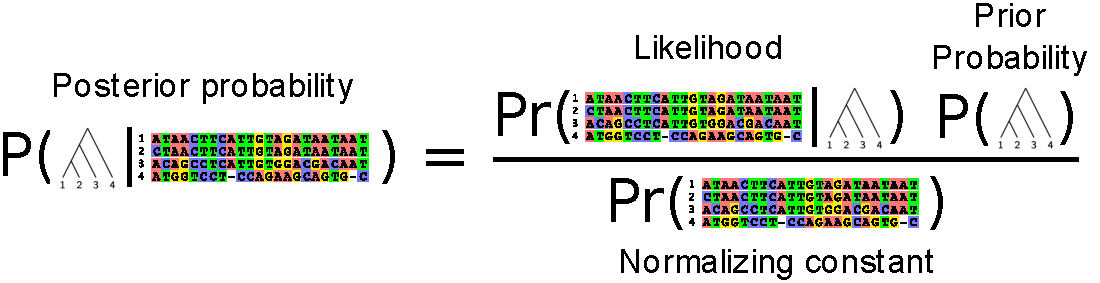
\includegraphics[width=\textwidth]{../images/PosteriorProbability}

\end{centering}

\medskip{}

This is known as the \textbf{Posterior probability} of the tree. Another method of reconstructing the evolutionary history is then to find the tree that has the \textbf{Maximum Posterior probability}.

\end{frame}
